\documentclass[12pt]{article}
\usepackage[a4paper, margin=1in, headheight=14pt]{geometry}
\usepackage[utf8]{inputenc}
\usepackage[spanish]{babel}
\usepackage{tabularx}
\usepackage{graphicx}
\usepackage{float}
\usepackage{setspace}
\usepackage{anyfontsize}
\usepackage[toc,page]{appendix} % Remove toc,page to render wo appendix
\usepackage{hyperref}
\usepackage[table]{xcolor}
\usepackage{fancyhdr}
\usepackage{nameref}
\usepackage{datetime}
\usepackage{tikz}
\usepackage[11pt]{moresize}
\usepackage{enumerate}
\usepackage{etoolbox}


\usetikzlibrary{calc}
\newcommand\HRule{\rule{\textwidth}{1pt}}


\pagestyle{fancy}
\fancyhf{}
\fancyhead[LE,RO]{Grupo 4}
\fancyhead[RE,LO]{\nombredelproyecto}
\fancyfoot[CE,CO]{\leftmark}
\fancyfoot[LE,RO]{\thepage}

\renewcommand{\headrulewidth}{2pt}
\renewcommand{\footrulewidth}{1pt}



\newcommand{\nombredelproyecto}{\textbf{Diagramas de secuencia y de clases GUI}}
\setcounter{secnumdepth}{4}
\makeatletter
\renewcommand{\paragraph}{\@startsection{paragraph}{4}{0ex}%
    {-3.25ex plus -1ex minus -0.2ex}%
    {1.5ex plus 0.2ex}%
    {\normalfont\normalsize\bfseries}}
\makeatother

\title{\nombredelproyecto} 
\author{Jesús Abajo Magro \\
Alejandro Díaz Blázquez \\
Javier Fernández Gamo \\
Andrés Galbán Méndez \\
Alejandro Gómez Molano \\
Jaime Millán Ibáñez Archilla \\
Rodrigo Sosa Saez \\
Alejandro Barrachina Argudo}


\date{\today}

\begin{document}
\begin{titlepage}


    \makeatletter
    \centering
    \vspace*{6\baselineskip}

    %------------------------------------------------
    %	Title
    %------------------------------------------------


    {\huge \underbar{\nombredelproyecto}\par} % Title

    %------------------------------------------------
    %	Subtitle
    %------------------------------------------------

    Ingeniería del software\\
    Ingeniería informática e ingeniería de computadores

    \vspace*{3\baselineskip} % Whitespace under the subtitle


    \begin{figure}[H]
        \centering
        
\includegraphics[width=0.5\textwidth]{images/Banqueo.png}
    \end{figure}
    %------------------------------------------------
    %	Editor(s)
    %------------------------------------------------


    \vspace{0.75\baselineskip} % Whitespace before the editors
    \begin{flushright}
        \small\@author\\ % Editor list
    \end{flushright}


    \vspace{0.5\baselineskip} % Whitespace below the editor list


    \vfill % Whitespace between editor names and publisher logo

    \vspace{0.3\baselineskip} % Whitespace under the publisher logo

    2020 % Publication year
    \makeatother
\end{titlepage}

\tableofcontents
\newpage

\section*{Introducción} %INTRODUCCION
En este documento se muestran los diagramas de secuencia y los diagramas de clase de las interfaces gráficas de la aplicación "Banqueo".

\section{Interfaces Gráficas} %INTERFACES GRAFICAS
En esta sección se muestran los diagramas de clases de las interfaces gráficas de la aplicación, con sus respectivos componentes.

\subsection{Interfaz Gráfica Cuentas}
\begin{figure}[H]
    \centering
    
\includegraphics[width=0.8\textwidth]{images/InterfazGraficaCuentas1.png}
\end{figure}

\subsection{Interfaz Gráfica Tarjetas}
\begin{figure}[H]
    \centering
    
\includegraphics[width=0.8\textwidth]{images/IntefazGraficaTarjetas1.png}
\end{figure}

\subsection{Interfaz Gráfica Prestamos}
\begin{figure}[H]
    \centering
    
\includegraphics[width=0.8\textwidth]{images/InterfazGraficaPrestamos_1.png}
\end{figure}

\subsection{Interfaz Gráfica Usuarios}
\begin{figure}[H]
    \centering
    
\includegraphics[width=0.8\textwidth]{images/InterfazGraficaUsuarios1.png}
\end{figure}

\newpage
\section{Diagramas de secuencia} %DIAGRAMAS DE SECUENCIA
En esta sección se muestran los diagramas de secuencia de los 4 subsistemas que existen en la aplicación: Usuarios, Cuentas, Préstamos y Tarjetas.
\subsection{Iniciar sesión}
\begin{figure}[H]
    \centering
    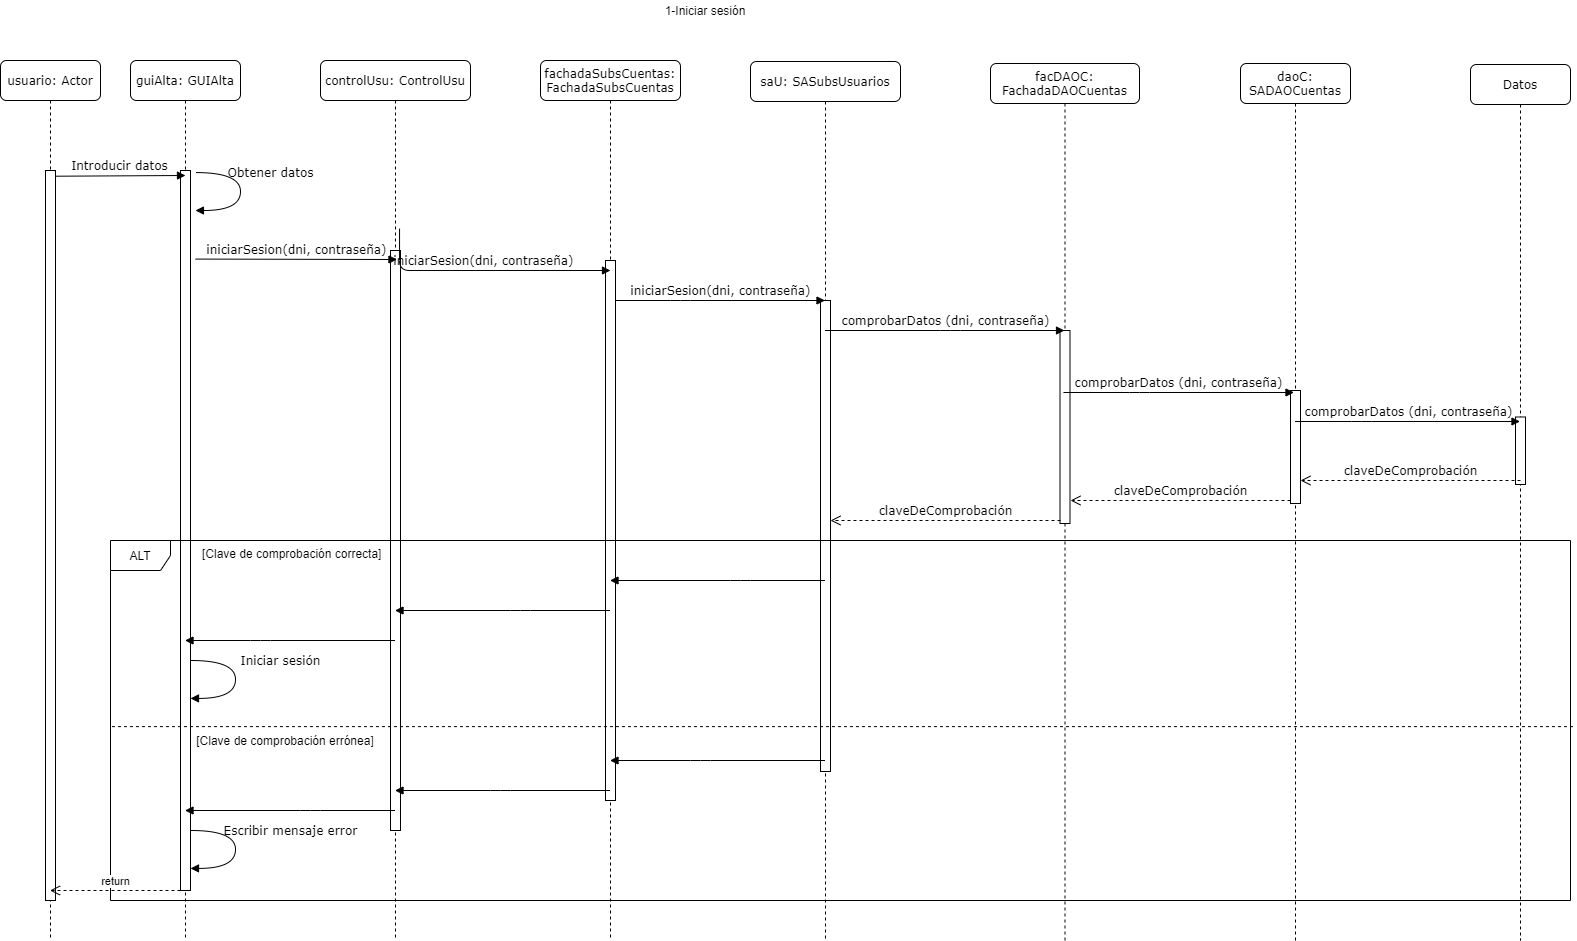
\includegraphics[width=0.8\textwidth]{images/iniciar_sesion.png}
\end{figure}
\subsection{Cerrar sesión}
\begin{figure}[H]
    \centering
    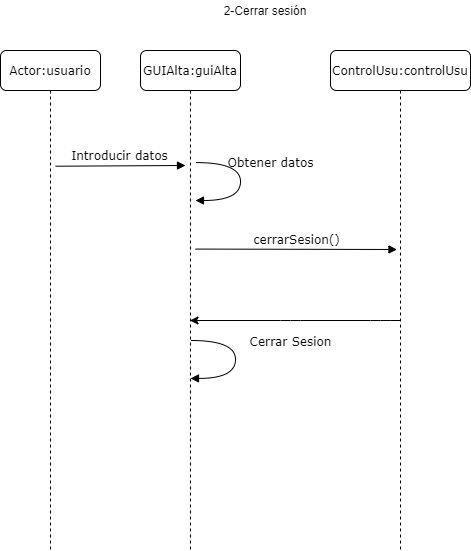
\includegraphics[width=0.4\textwidth]{images/2-Cerrar_sesion.png}
\end{figure}
\subsection{Gestor crea cuenta cliente}
\begin{figure}[H]
    \centering
    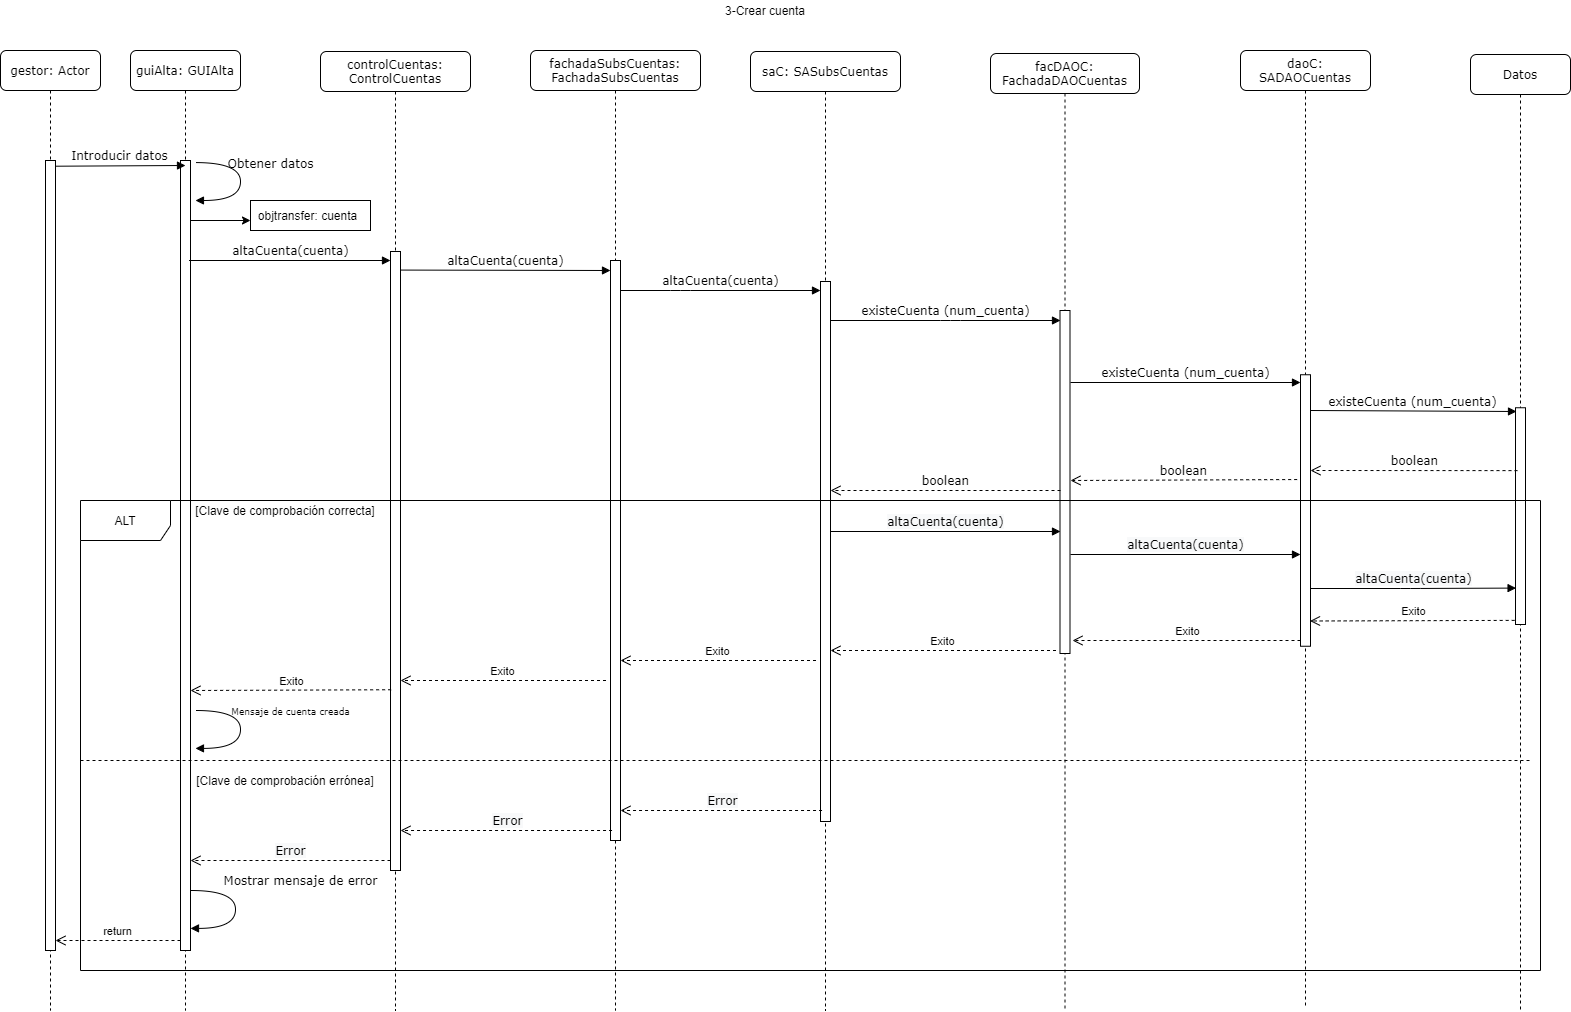
\includegraphics[width=0.8\textwidth]{images/crear_cuenta.png}
\end{figure}
\subsection{Gestor elimina cuenta cliente}
\begin{figure}[H]
    \centering
    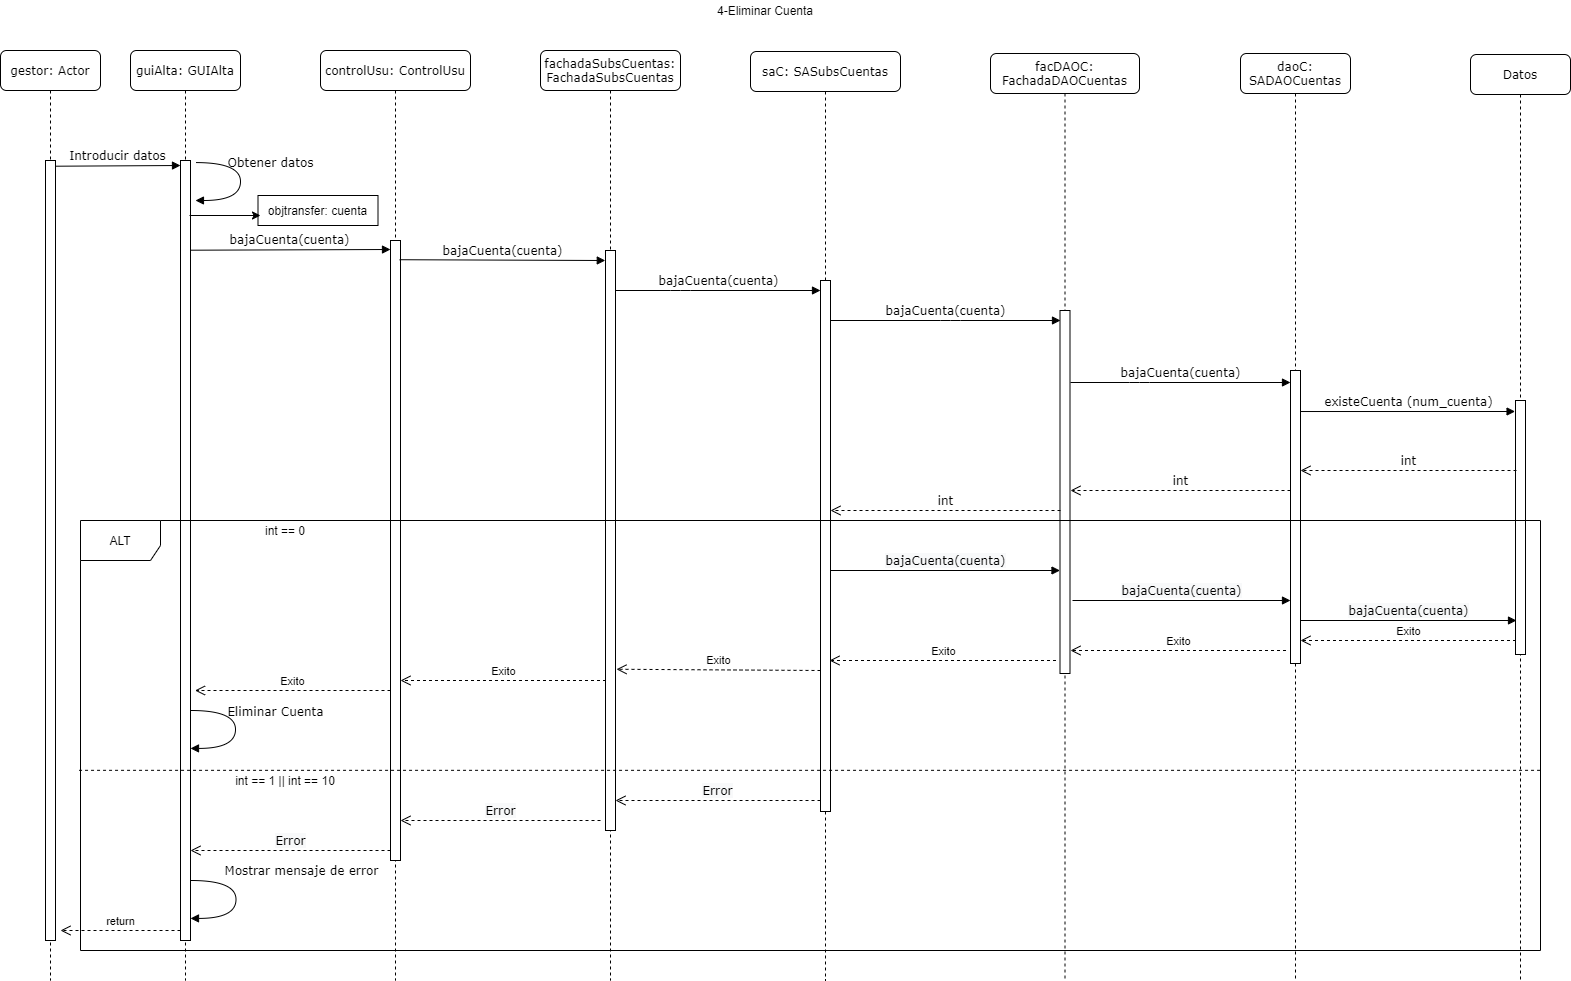
\includegraphics[width=0.8\textwidth]{images/eliminar_cuenta.png}
\end{figure}

\subsection{Gestor selecciona cliente}
\begin{figure}[H]
    \centering
    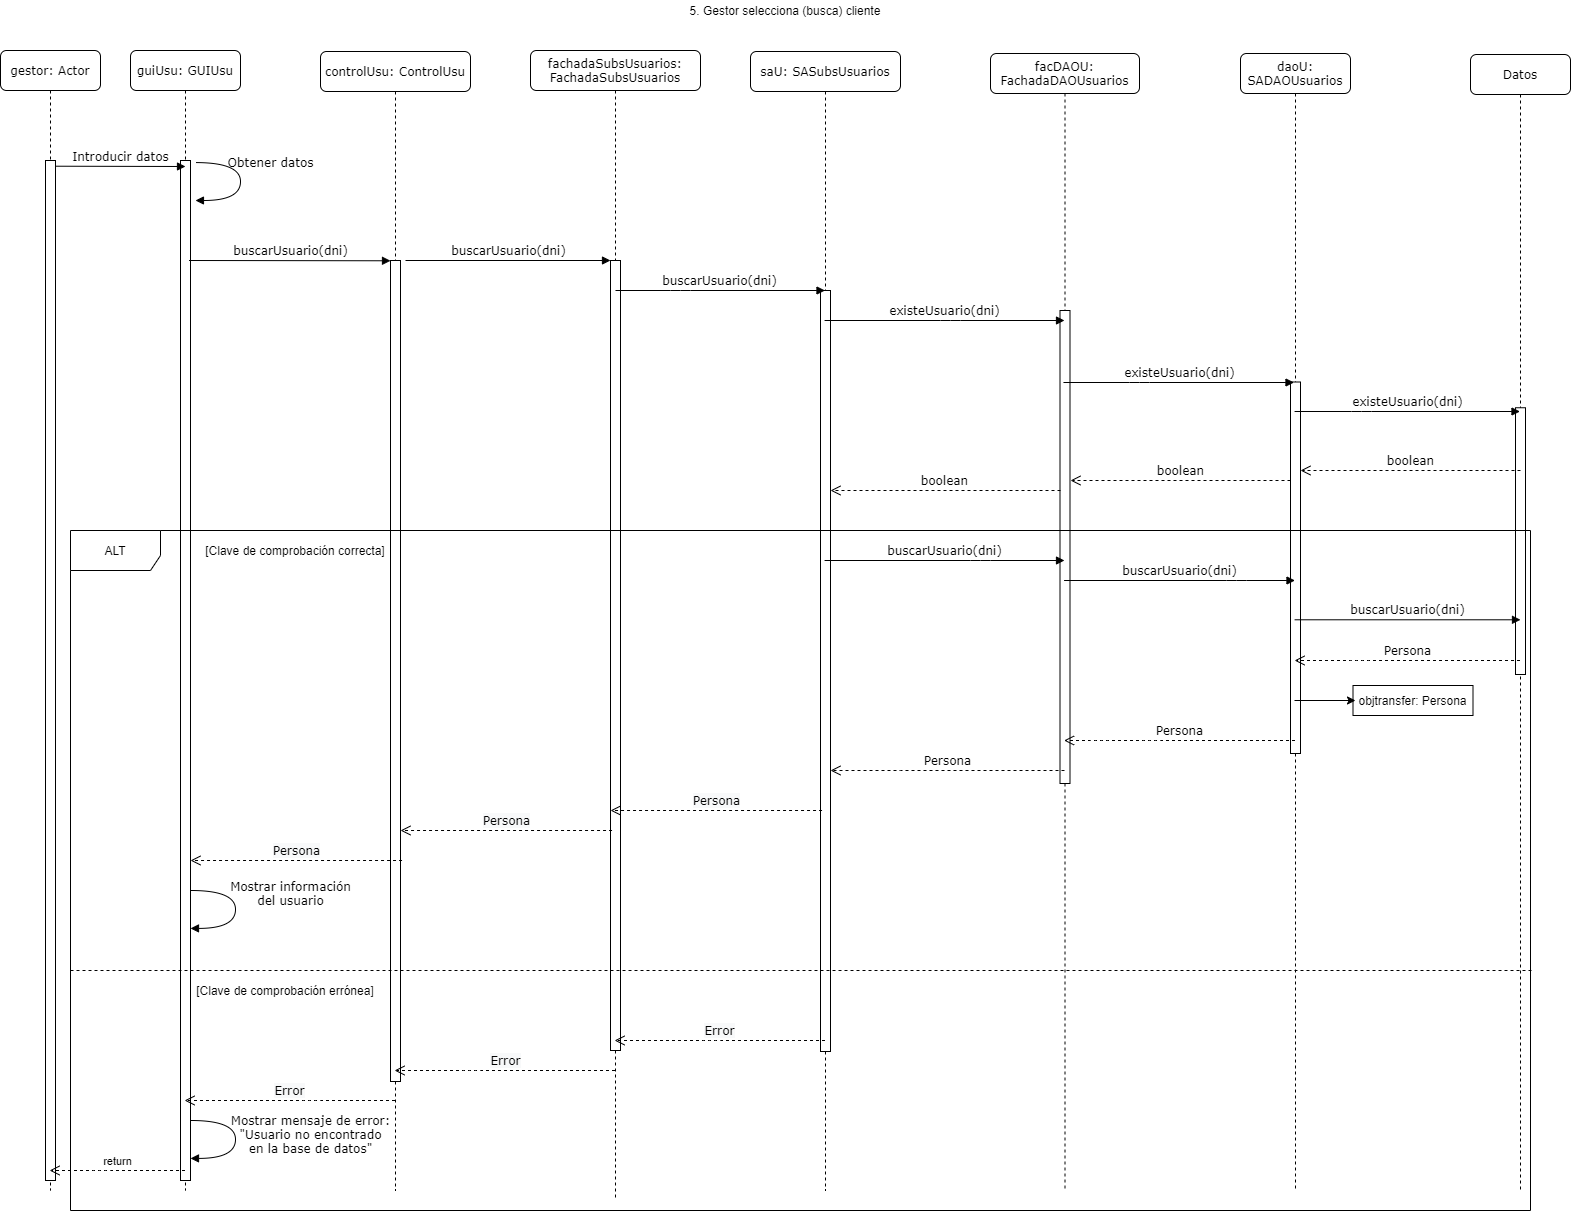
\includegraphics[width=0.8\textwidth]{images/gestor_selecciona_cliente_consultar_5.png}
\end{figure}

\subsection{Cliente solicita préstamo}
\begin{figure}[H]
    \centering
    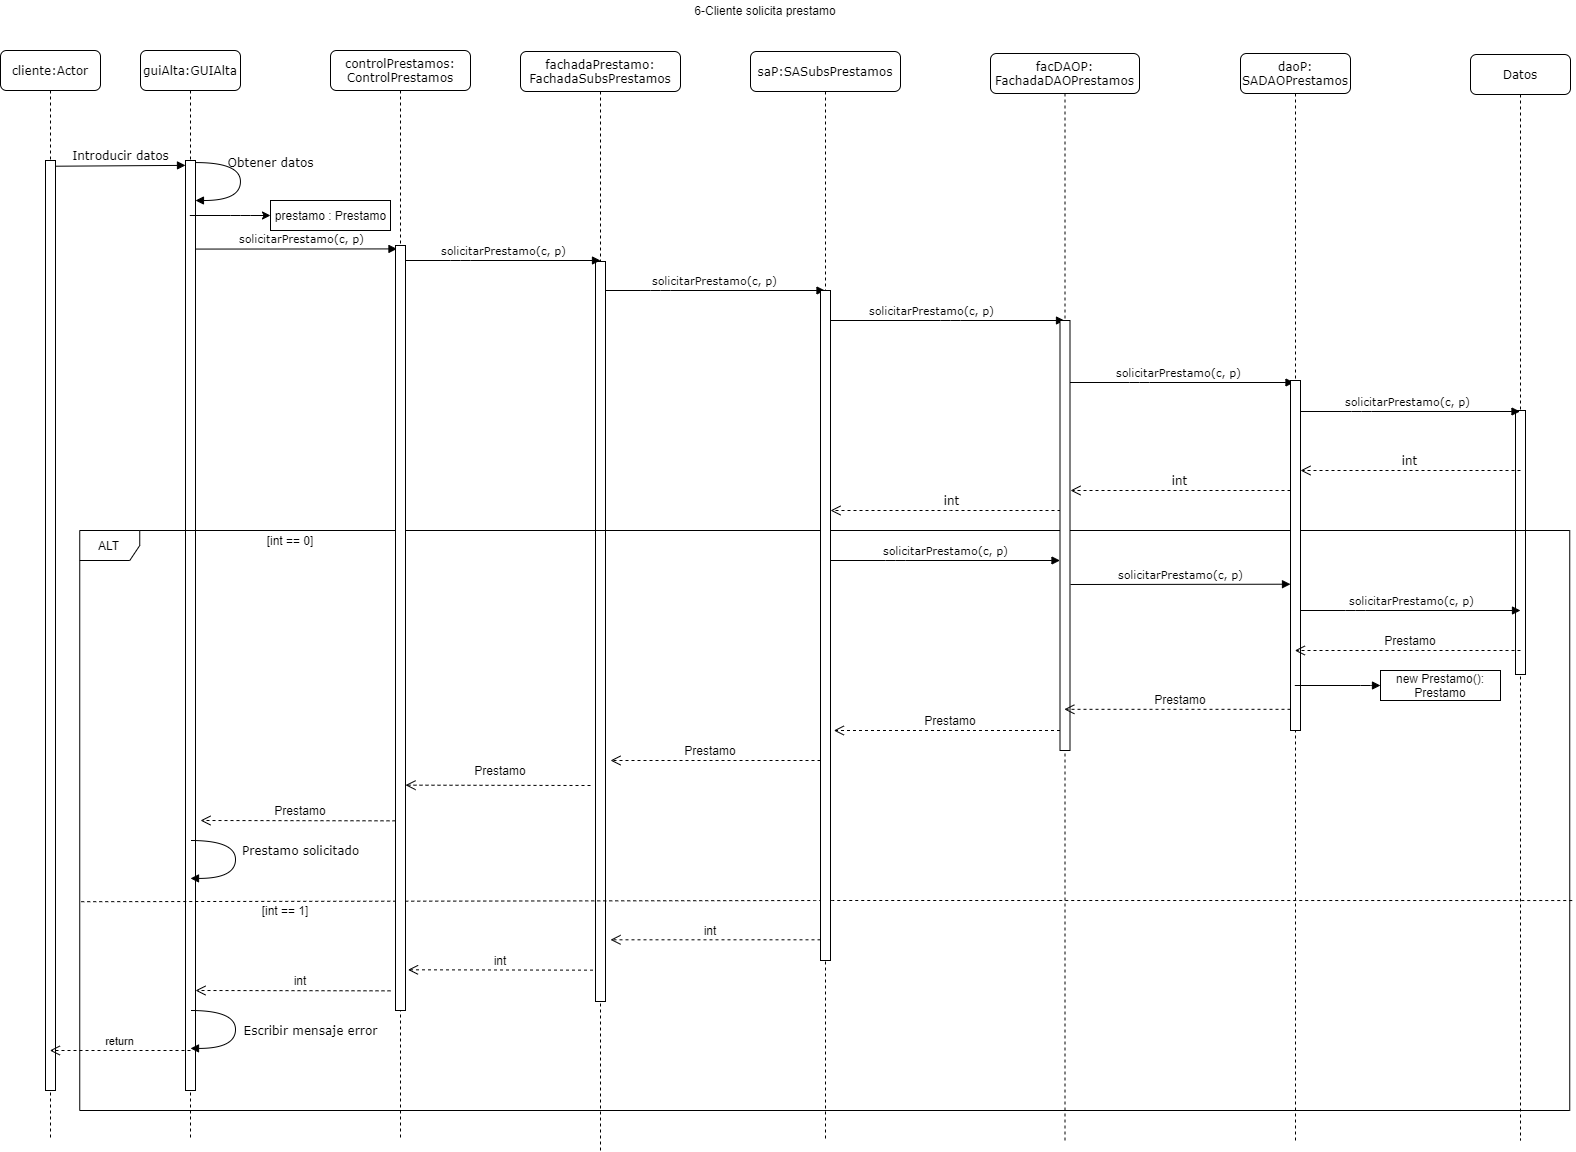
\includegraphics[width=0.8\textwidth]{images/ClienteSolicitaPrestamo2.png}
\end{figure}
\subsection{Modificar tarjeta}
\begin{figure}[H]
    \centering
    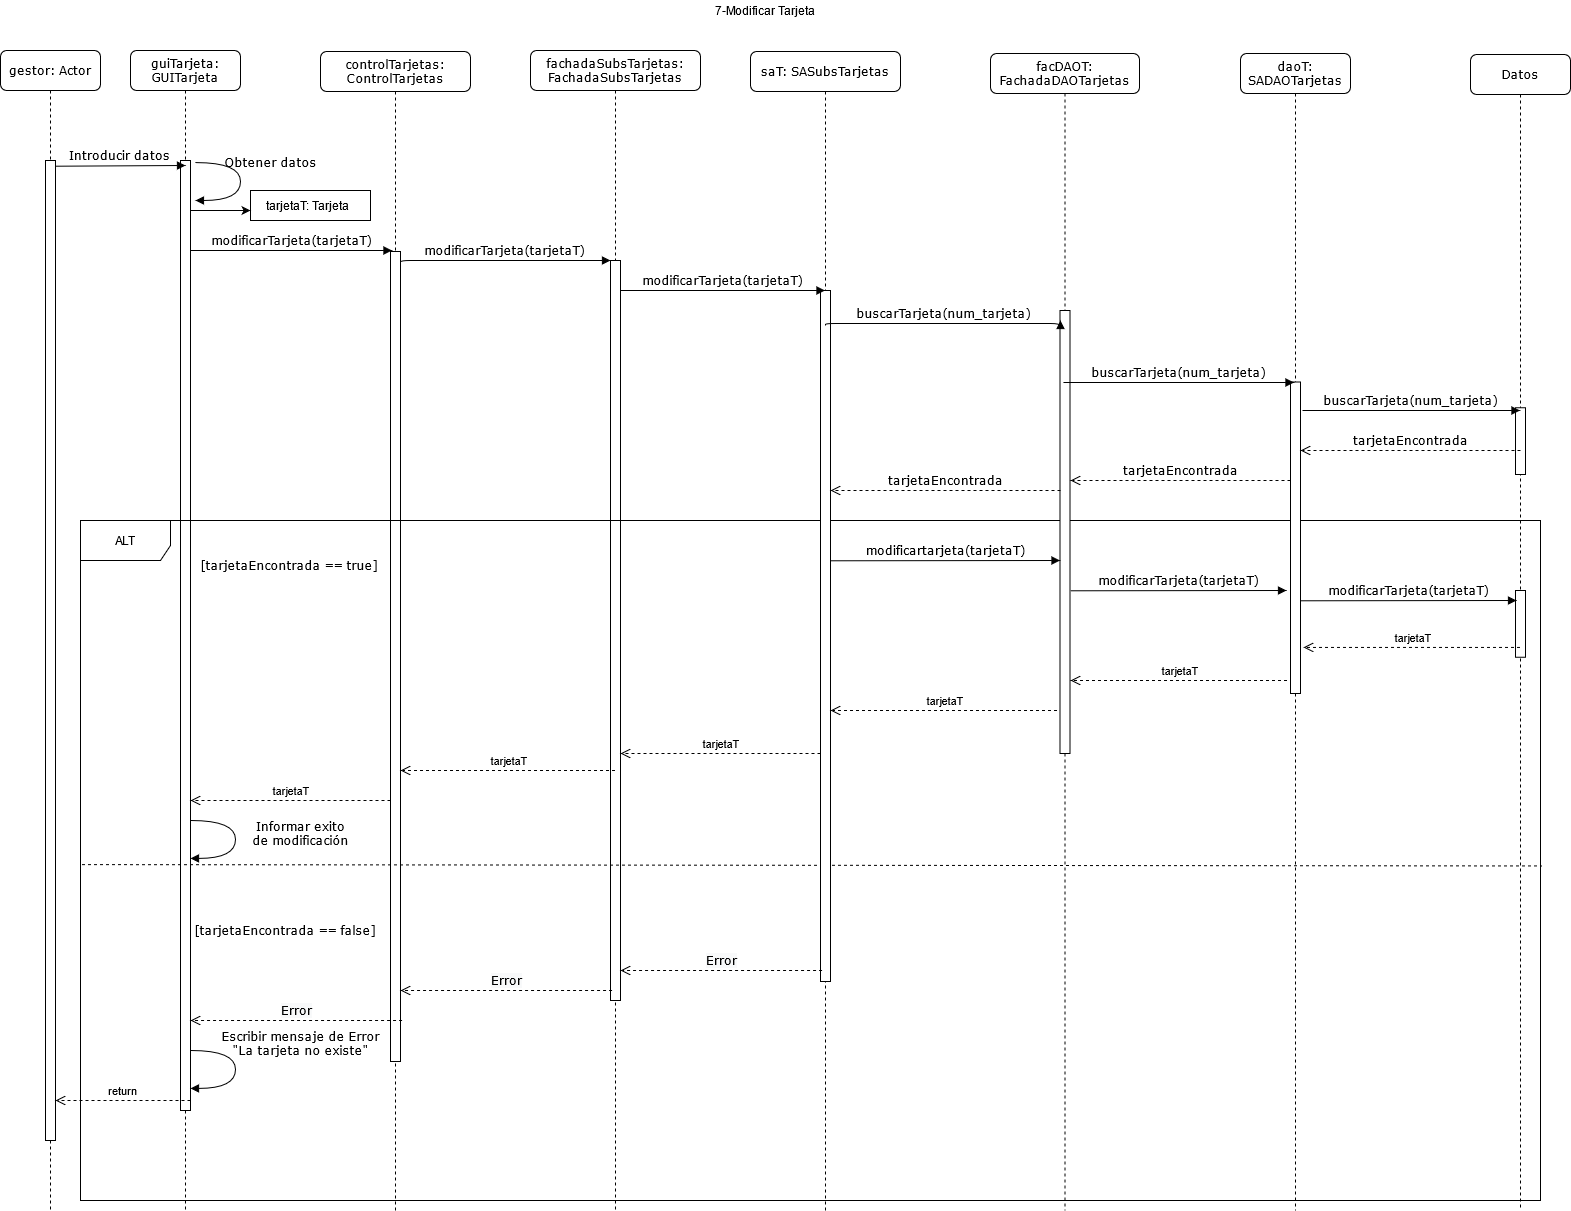
\includegraphics[width=0.8\textwidth]{images/7-Gestor_modifica_tarjeta.png}
\end{figure}
\subsection{Modificar cuenta}
\begin{figure}[H]
    \centering
    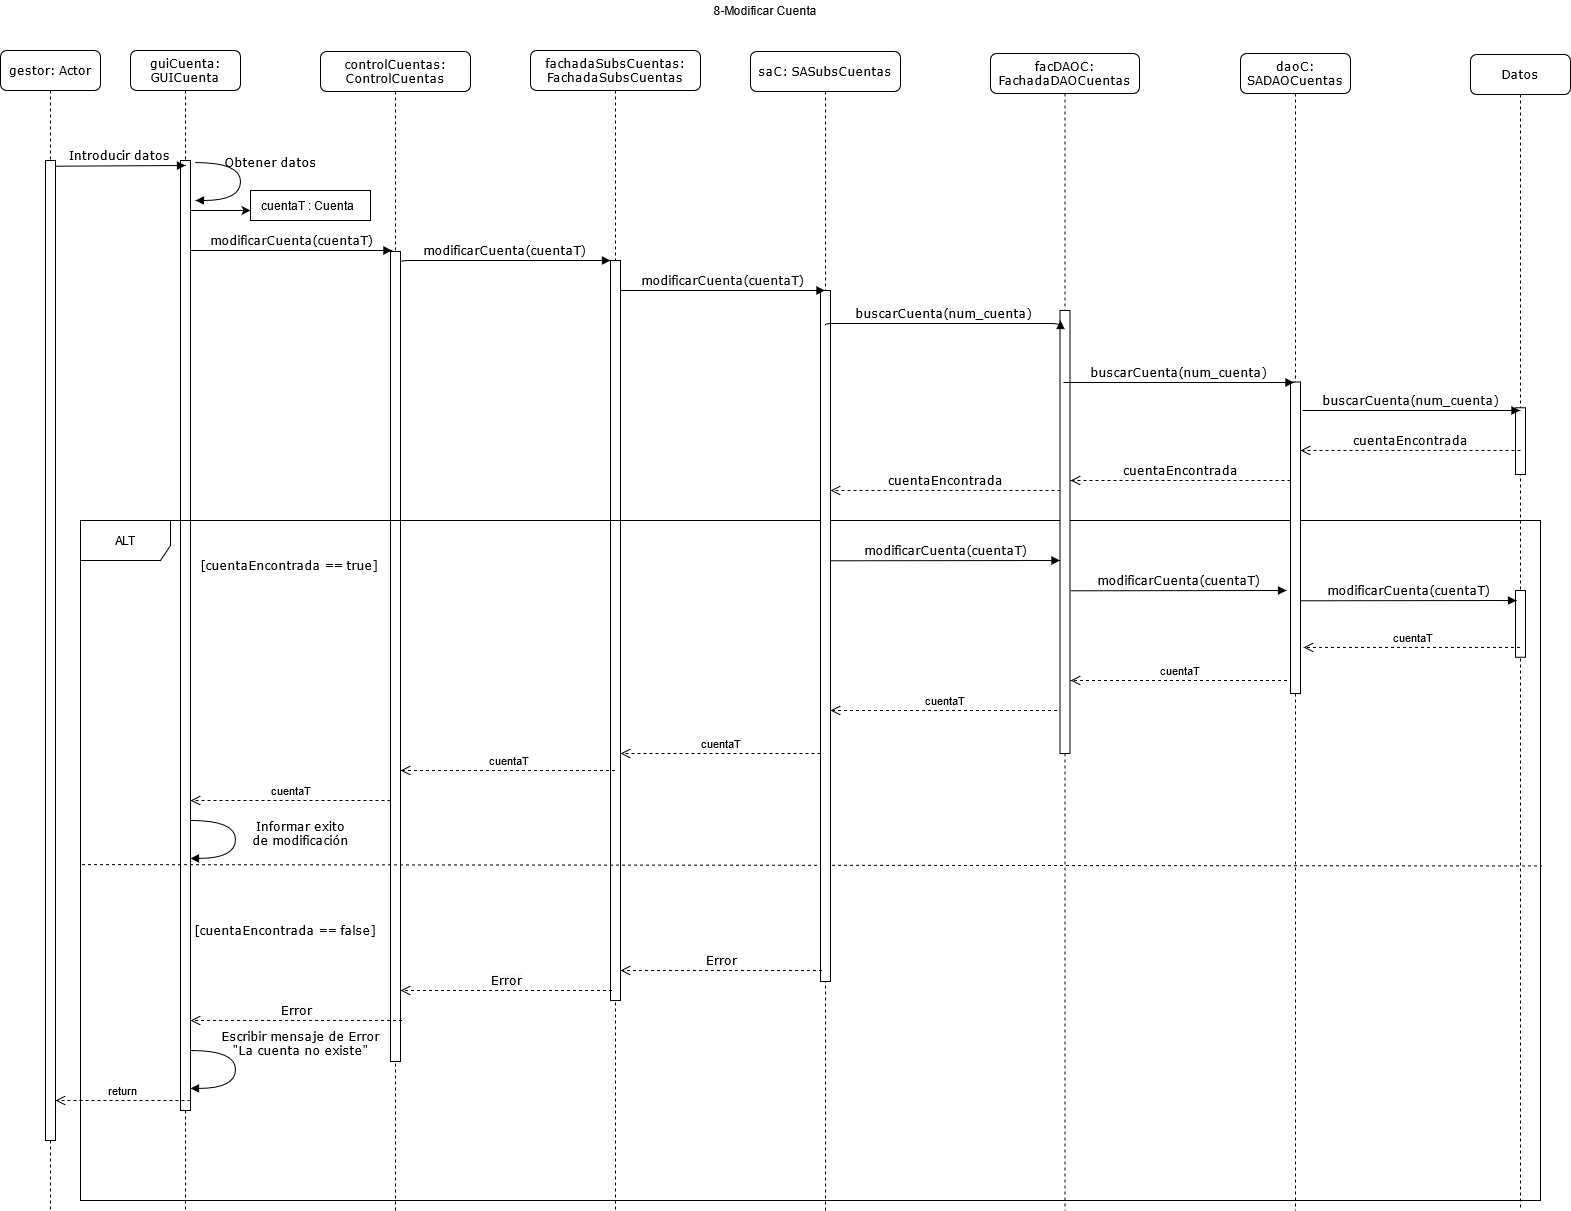
\includegraphics[width=0.8\textwidth]{images/8-Gestor_modifica_cuenta.png}
\end{figure}
\subsection{Modificar préstamo}
\begin{figure}[H]
    \centering
    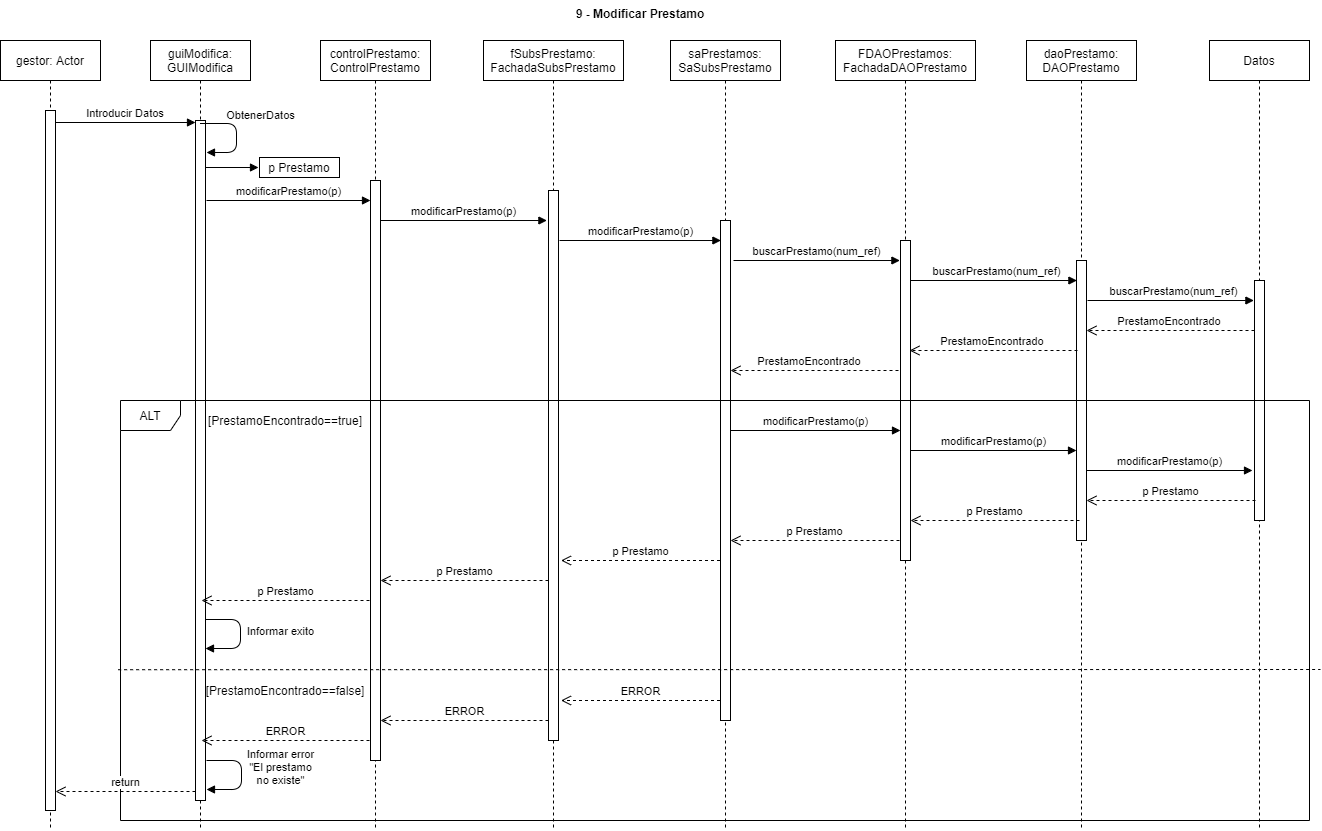
\includegraphics[width=0.8\textwidth]{images/9._GestorModificaPrestamo.png}
\end{figure}
\subsection{Modificar usuario}
\begin{figure}[H]
    \centering
    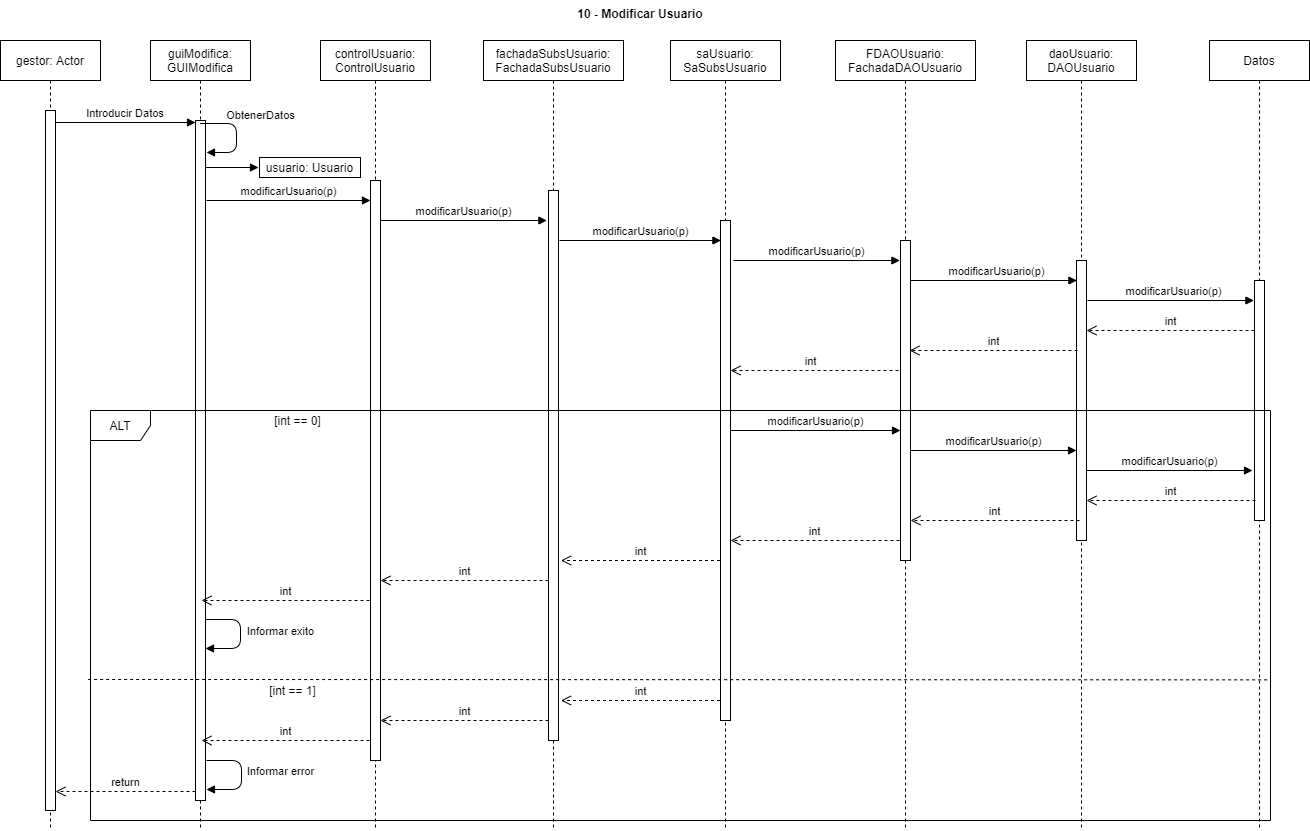
\includegraphics[width=0.8\textwidth]{images/10._ModificarUsuario.png}
\end{figure}
\subsection{Consultar cuenta}
\begin{figure}[H]
    \centering
    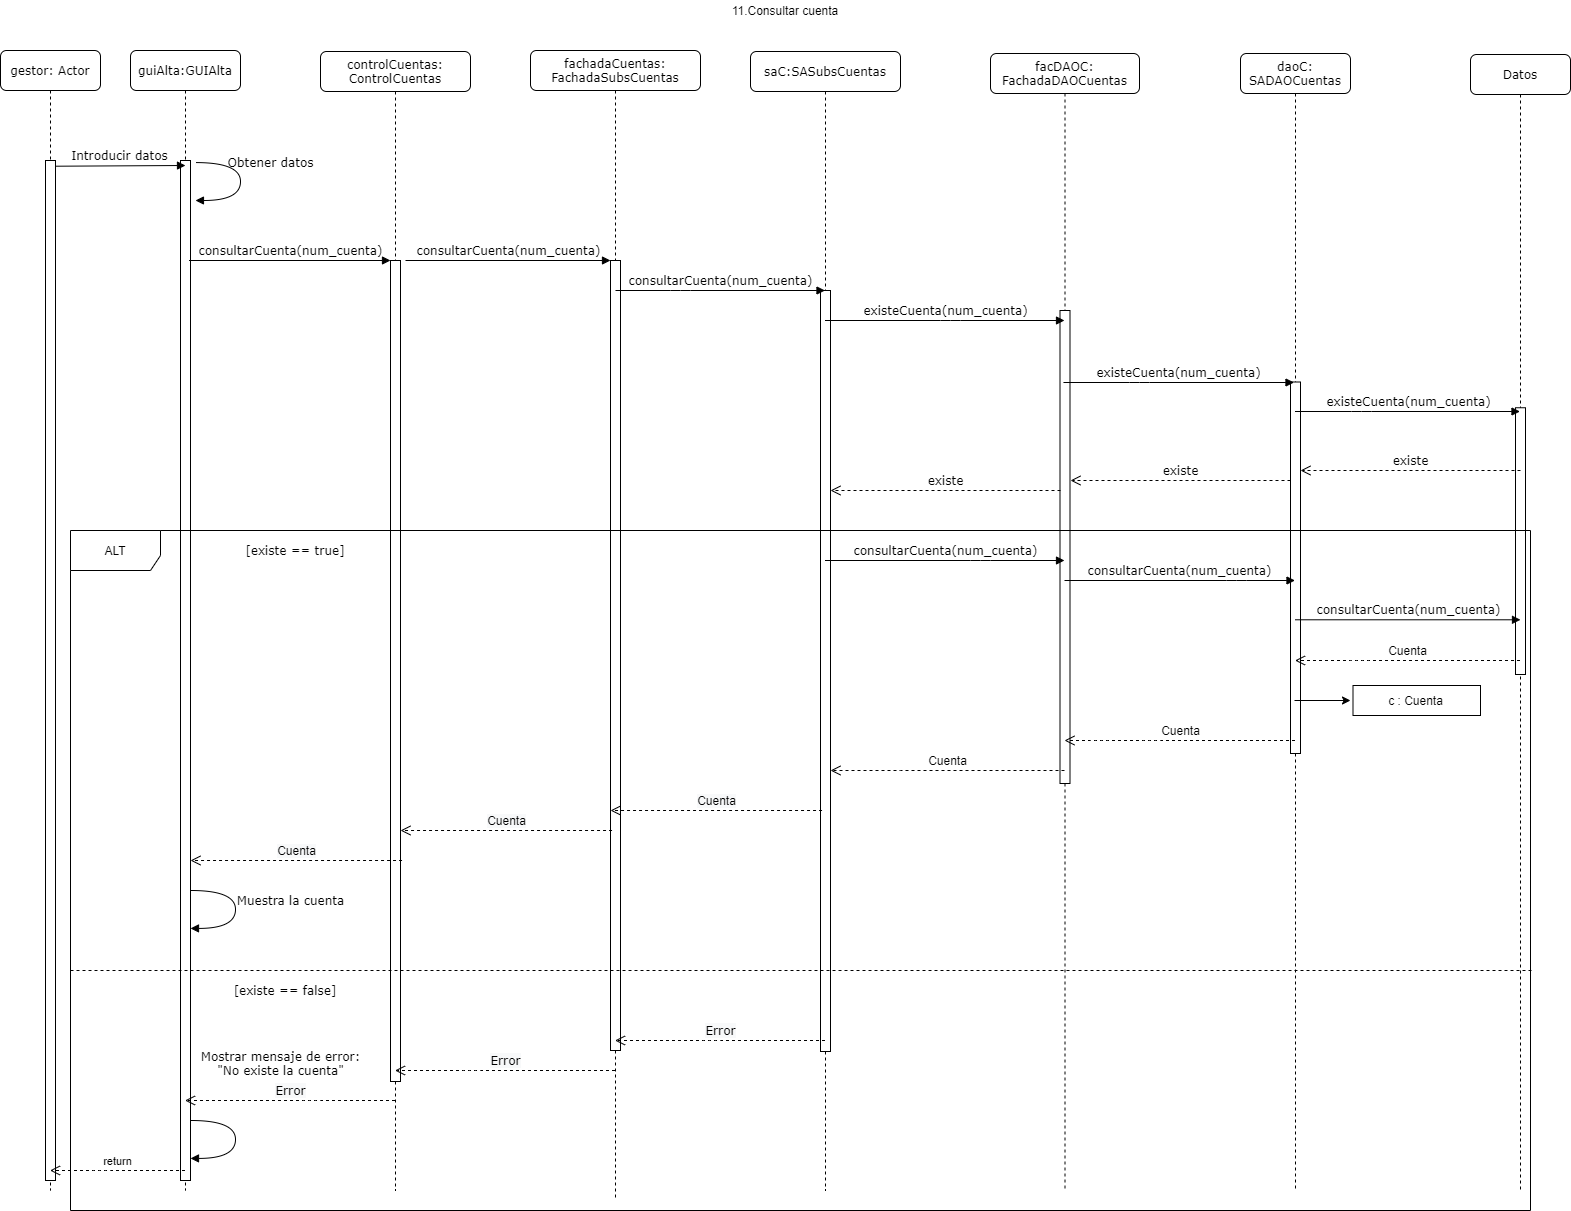
\includegraphics[width=0.8\textwidth]{images/ConsultaCuenta.png}
\end{figure}
\subsection{Consultar préstamo}
\begin{figure}[H]
    \centering
    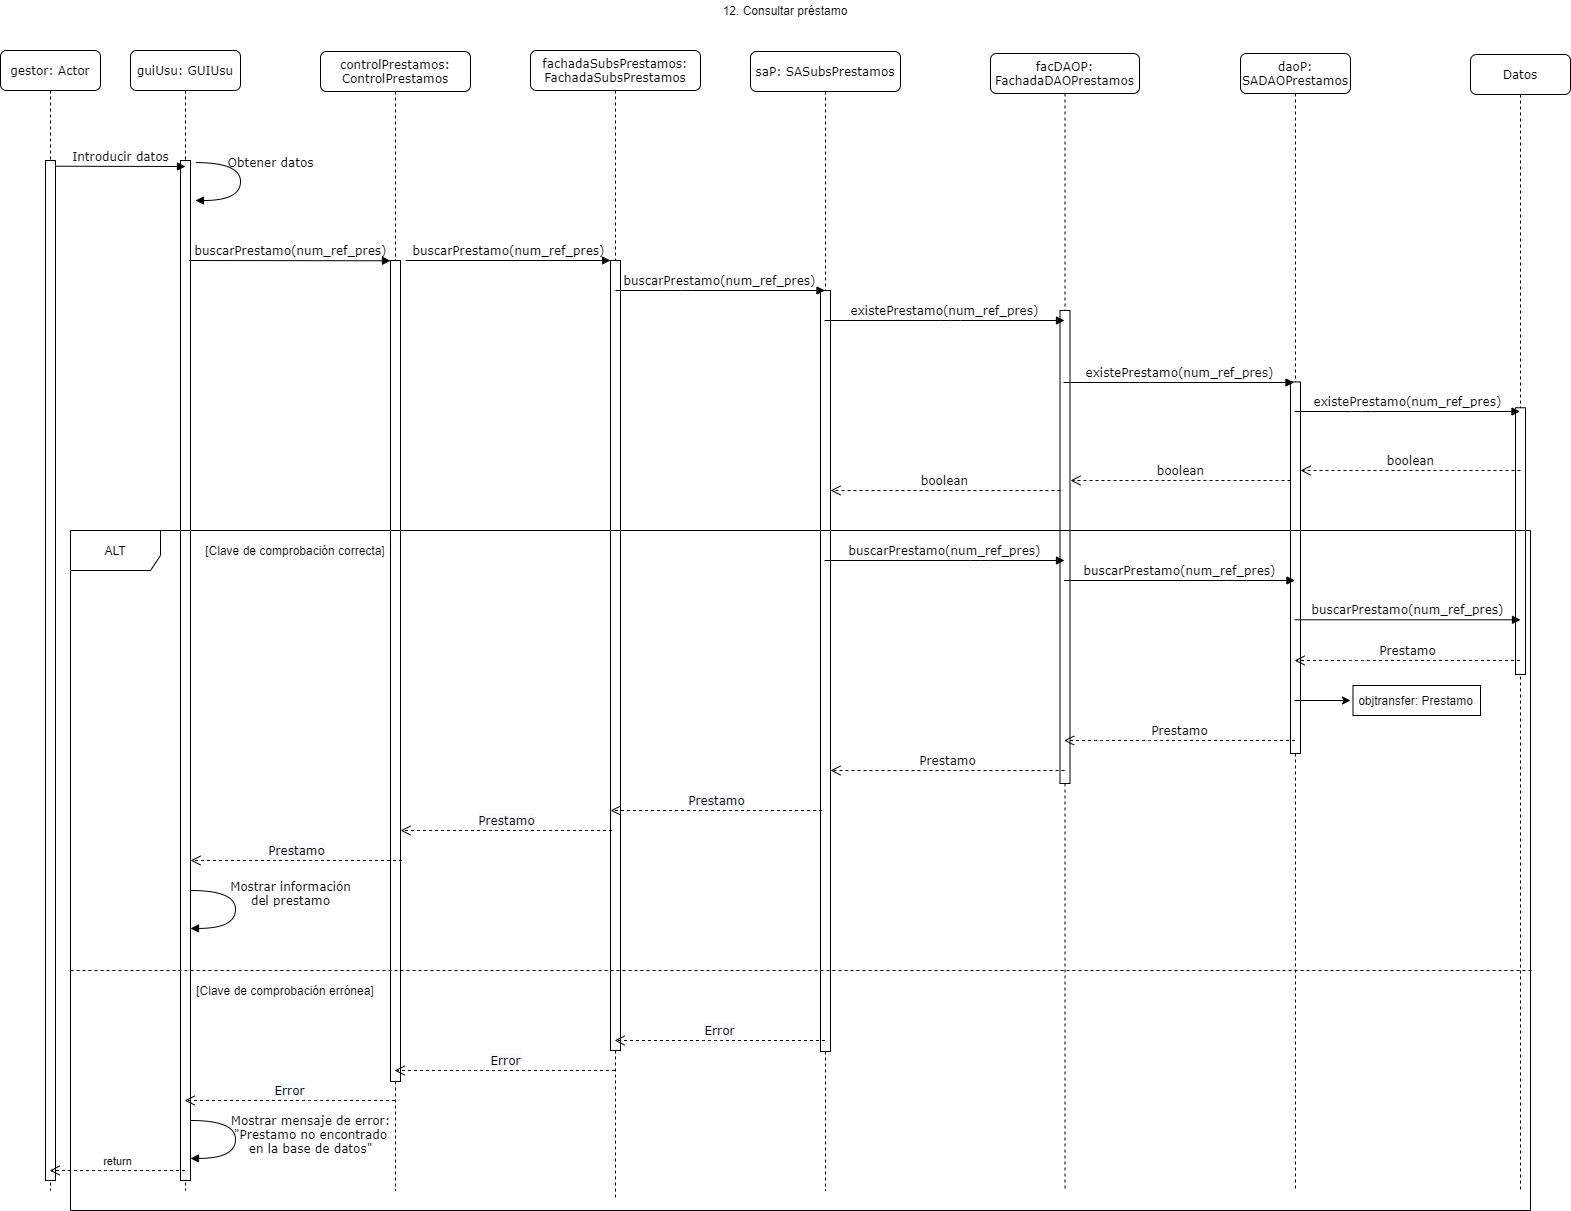
\includegraphics[width=0.8\textwidth]{images/consultar_prestamo.png}
\end{figure}
\subsection{Consultar tarjeta}
\begin{figure}[H]
    \centering
    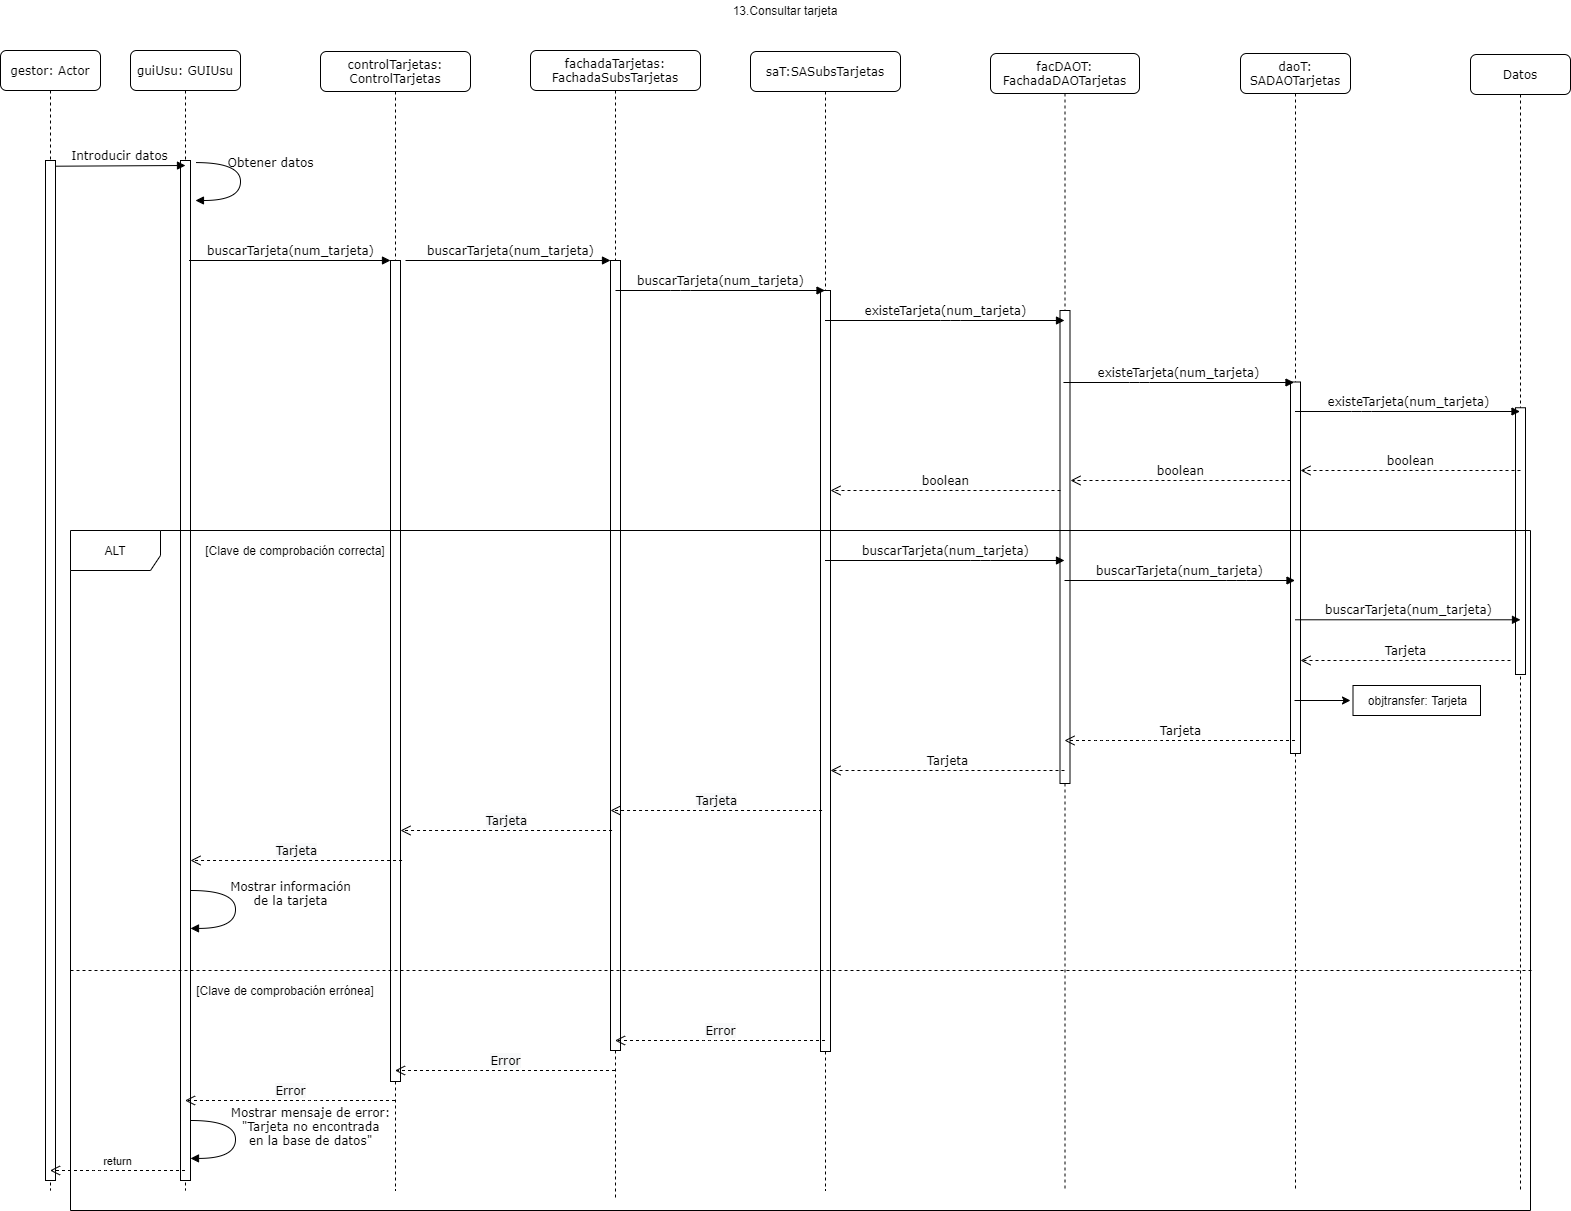
\includegraphics[width=0.8\textwidth]{images/consultarTarjeta.png}
\end{figure}
\subsection{Gestor crea tarjeta}
\begin{figure}[H]
    \centering
    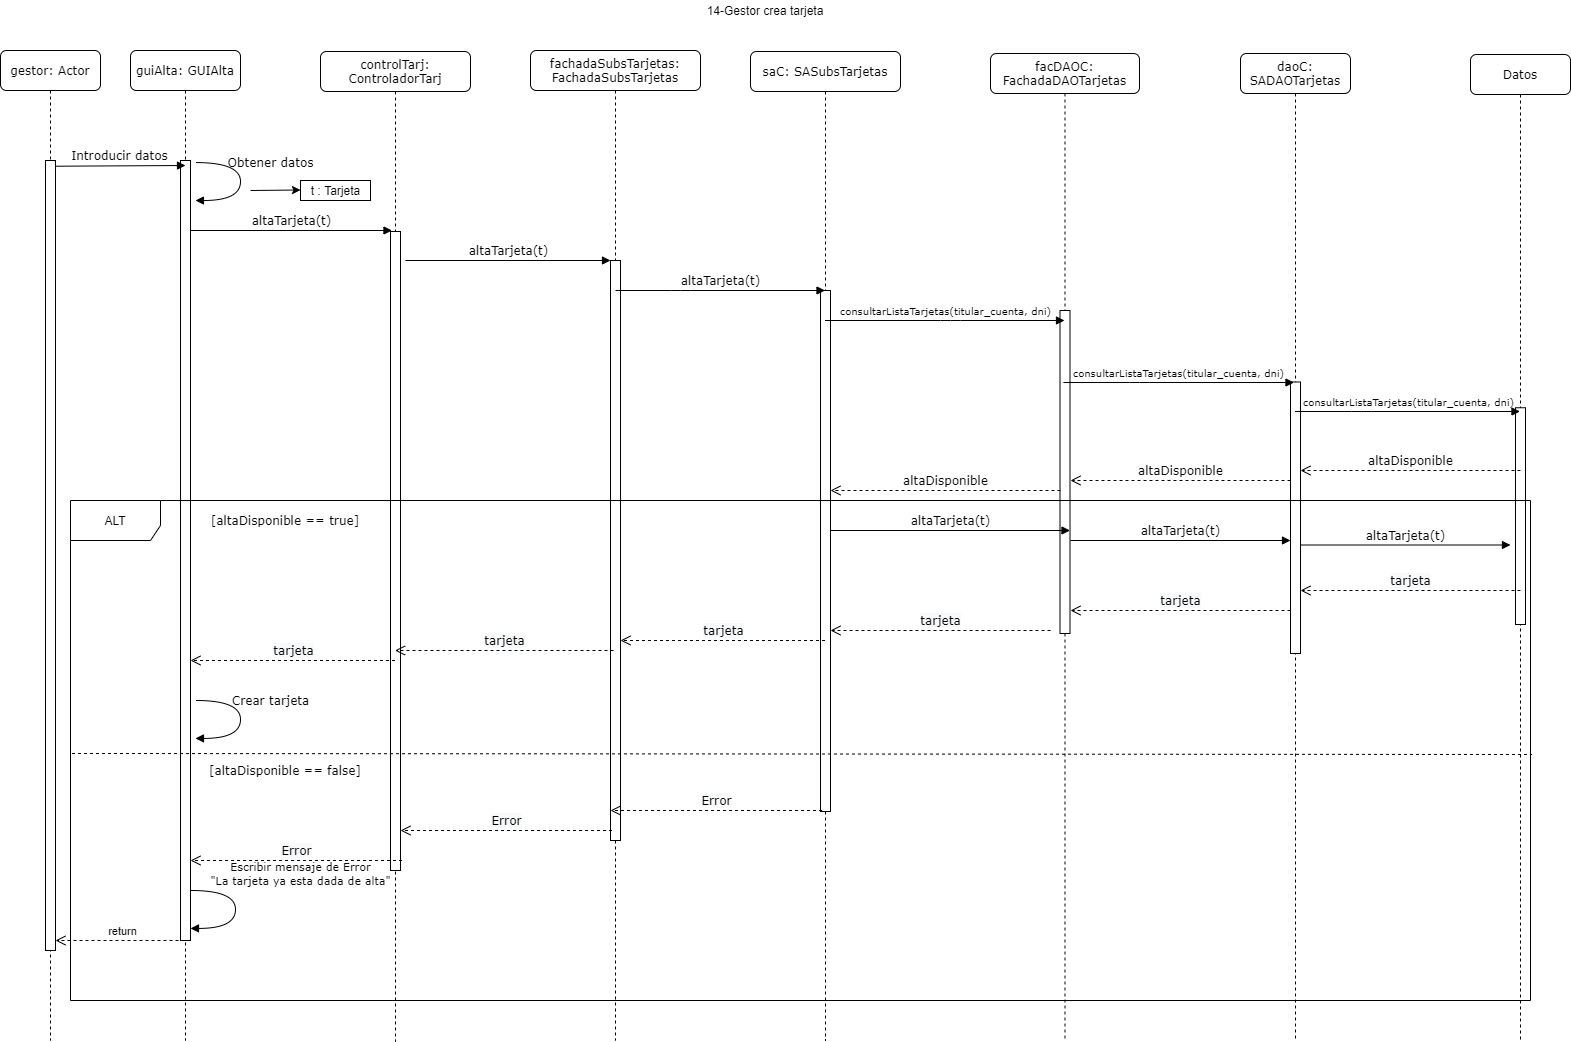
\includegraphics[width=0.8\textwidth]{images/14-Gestor_crea_tarjeta.png}
\end{figure}
\subsection{Gestor elimina tarjeta}
\begin{figure}[H]
    \centering
    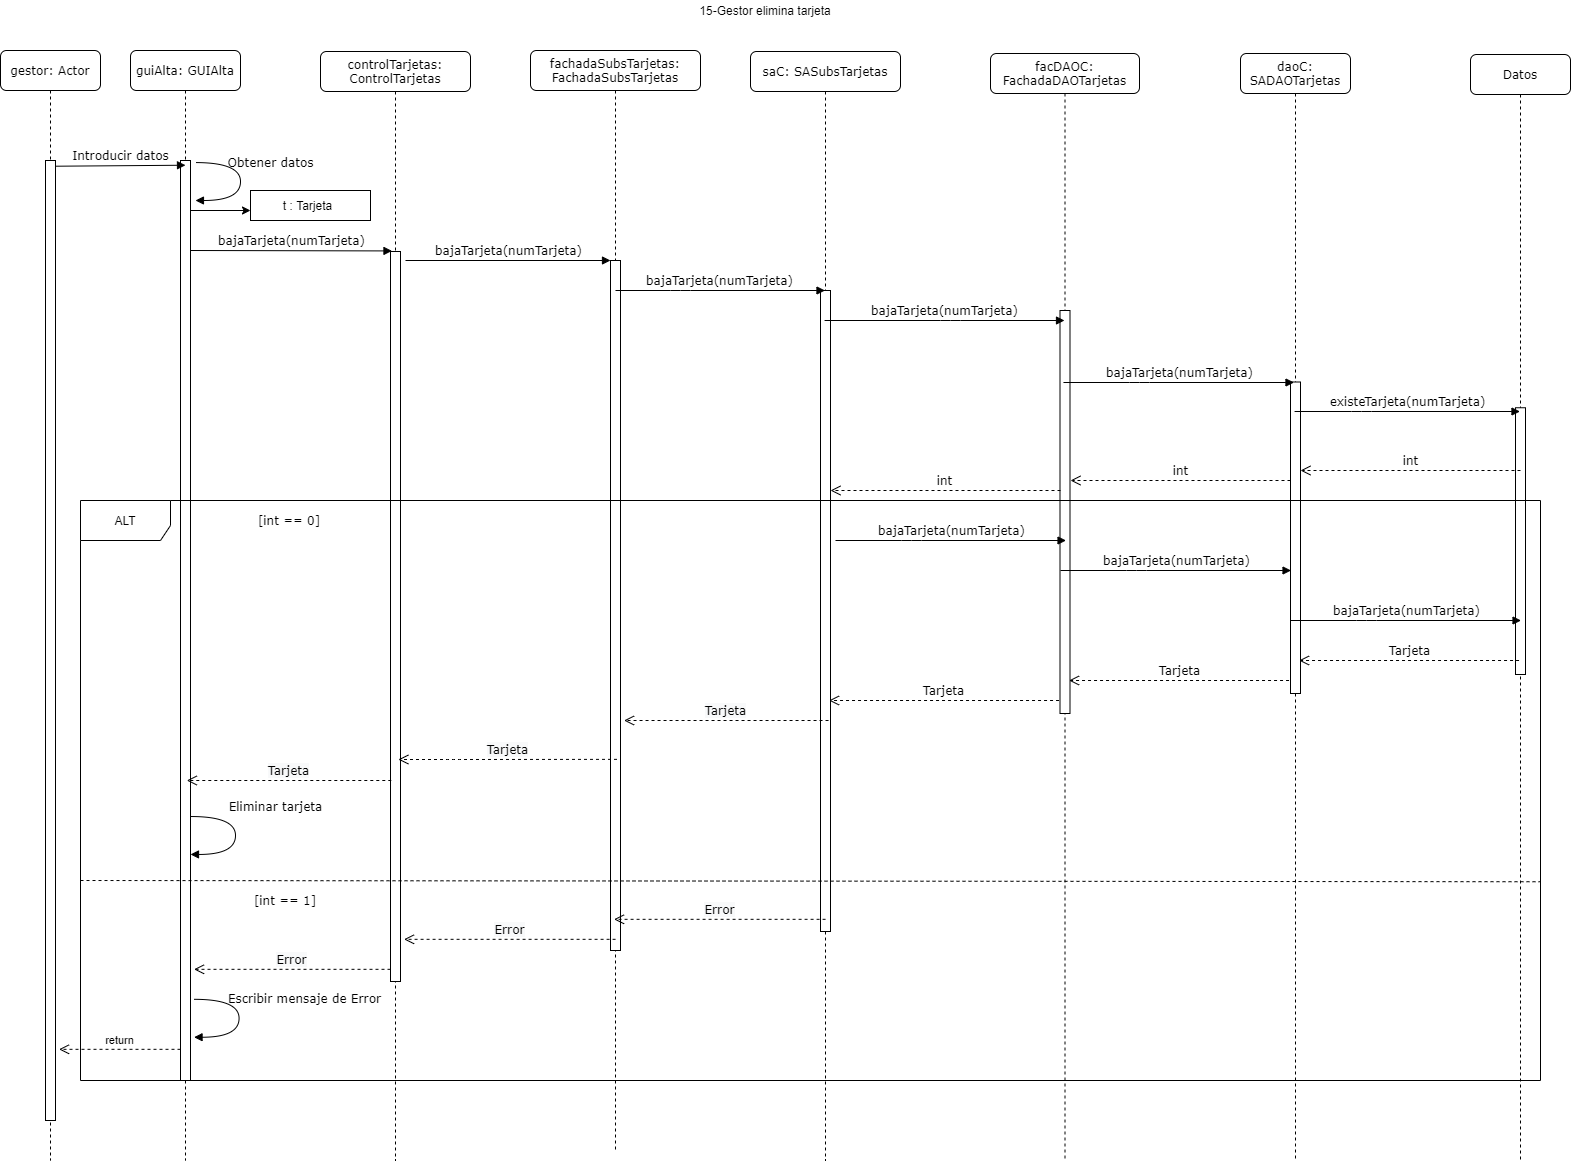
\includegraphics[width=0.8\textwidth]{images/15-Gestor_elimina_tarjeta.png}
\end{figure}
\end{document}
